\documentclass[conference]{IEEEtran}
\IEEEoverridecommandlockouts

\usepackage{cite}
\usepackage{amsmath, amssymb, amsfonts}
\usepackage{algorithmic}
\usepackage{graphicx}
\usepackage{textcomp}
\usepackage{xcolor}
\def\BibTeX{{\rm B\kern-.05em{\sc i\kern-.025em b}\kern-.08em
    T\kern-.1667em\lower.7ex\hbox{E}\kern-.125emX}}

\begin{document}

\title{Relief Link Research Report\\
{\footnotesize \textsuperscript{*}2024 Spring Introduction to FinTech, National Taiwan University}
\thanks{2024 Spring Introduction to FinTech, National Taiwan University}
}

\author{\IEEEauthorblockN{1\textsuperscript{st} CHIH-HAO LIAO}
    \IEEEauthorblockA{
        \textit{School of Forestry and Resource Conservation} \\
        \textit{Graduate Institute of Biomedical Electronics and Bioinformatics} \\
        \textit{National Taiwan Universiry}\\
        Taipei, Taiwan \\
        R11625015@ntu.edu.tw}
}

\maketitle
\thispagestyle{plain}
\pagestyle{plain}

\begin{abstract}
    The Relief Link initiative integrates various cutting-edge technologies to provide timely aid in the aftermath of natural disasters. By leveraging Chainlink oracles for real-time monitoring and automated transactions, coupled with PredictHQ's API for disaster impact analysis, the platform ensures swift delivery of assistance within a specific radius of users' locations. Worldcoin authentication enhances security and prevents fraud, while Unlimit facilitates convenient access to fiat currency options. Additionally, collaboration with Nouns DAO enhances user experience through unique avatars, fostering a sense of community. This research paper comprehensively analyzes the technical implementation of Relief Link, assesses its broad applicability and feasibility, and offers recommendations for its optimization and expansion.
\end{abstract}

\begin{IEEEkeywords}
    Relief Link, ETHGlobal, Chainlink Oracles, Worldcoin, PredictHQ, Unlimit
\end{IEEEkeywords}

\section{Introduction}
This is the final research report of the Introduction to FinTech Course (Spring 2024, National Taiwan University). This research report aims to thoroughly examine the technical implementation details of the Relief Link project, evaluate its wide-ranging applicability and feasibility, and offer informed recommendations based on our findings. Relief Link project is the winner of the Worldcoin - Best Public Goods Use Case and ETHGlobal - ETHGlobal Sydney Finalist, and the project aims to solve the problem of real-time disaster monitoring and automated distribution aid, ensuring timely delivery of aid and emergency relief materials to those affected communities within a specific radius after a disaster.

\section{Background}
One of the primary challenges in emergency relief operations is the effective allocation of limited relief materials to the impacted communities. This challenge is often exacerbated by issues such as the inability to accurately assess the demand and utility of relief materials and the potential for malicious actions by some stakeholders, leading to ad-hoc and inefficient distribution \cite{b1}. Consequently, establishing an unalterable and globally accessible record of relief needs and allocations is crucial for efficient management.

Relief Link is an innovative service designed to automatically distribute aid immediately after a disaster, leveraging blockchain technology for efficient and secure operations. The project integrates Chainlink oracles for real-time disaster monitoring and automated transactions, ensuring timely delivery of aid to those affected within a specific radius. The system attracts users, even those new to cryptocurrency, through account abstraction from Unlimit and third-party networks, allowing for convenient access to fiat currency options.

Relief Link uses Worldcoin for authentication to maintain system integrity and prevent fraud, ensuring that aid is distributed once per verified user. The Relief Link platform leverages PredictHQs API to track and analyze the impact of various natural disasters (such as floods, fires, and earthquakes) within 100 kilometers of the users registered location. This data is visualized on the website, providing insights into recent disaster trends in the Asia-Pacific region.

The platform integrates Chainlink oracles for real-time disaster monitoring and automated transactions, ensuring timely delivery of aid to those affected within a specific radius. The system attracts users, even those new to cryptocurrency, through account abstraction from Unlimit and third-party networks, allowing for convenient access to fiat currency options. Relief Link uses Worldcoin for authentication to maintain system integrity and prevent fraud, ensuring that aid is distributed once per verified user. The Relief Link platform leverages PredictHQs API to track and analyze the impact of various natural disasters (such as floods, fires, and earthquakes) within 100 kilometers of the users registered location. This data is visualized on the website, providing insights into recent disaster trends in the Asia-Pacific region.

\section{Methodology}
\subsection{Chainlink Oracles}
Chainlink oracles are a crucial component of the Relief Link platform. Chainlink is a blockchain initiative aimed at linking various networks and protocols via oracles, which are third-party services supplying smart contracts with external data. Since smart contracts cannot actively retrieve real-world data, the role of oracles here acts as API interfaces or intermediaries between blockchains and real-world information, connecting DeFi smart contracts on the blockchains with real-world data and enabling smart contracts to access and interact with external data. With the mechanism, Chainlink Oracles' objective is to support all blockchains, enabling the global transfer of data across different blockchains. In other words, Chainlink can successfully connect blockchains to the real world.

Chainlink, the leading platform for decentralized oracle systems, facilitates the transmission of real-world data to blockchains. It has developed a multi-node distributed information aggregator, akin to Bitcoin's mechanism, to ensure the provision of reliable and tamper-proof data for DeFi smart contracts on the blockchain. With its decentralized, secure, open-sourced, and reliable characteristics, Chainlink oracles are ideal for integration into the Relief Link platform.

In the Relief Link project, these oracles provide real-time data on natural disasters, allowing the system to monitor and respond to events promptly after verifying the reliability of the source data. The oracles collect information from various sources, such as weather stations and seismic sensors, and feed it into the Relief Link system. This data is then used to trigger automated transactions and distribute aid to affected areas. This integration ensures that aid distributions are triggered briskly and accurately when conditions meet predefined criteria, which is custom logic automation, offering transparency and reliability which are crucial for disaster response.

\subsection{Worldcoin(WLD)}
To ensure the integrity and fairness of aid distribution within the Relief Link platform, they have integrated Worldcoin's advanced identity verification technology. Worldcoin utilizes a unique system of iris biometric scanning through orb-shaped devices, which securely verifies the identity of each recipient.

The recipients are required to undergo an iris scan using Worldcoin's orb-shaped scanners, and the biometric data is then used to create a unique digital identity for each recipient, ensuring that each individual can only be registered once. Following the iris scan, a World ID is generated for each recipient. This World ID serves as a secure and reliable means of authentication, which can be used to verify the recipient's identity during the distribution of aid. To access their aid, recipients must provide their World ID and use the Worldcoin app. All personal data collected during this process is encrypted and stored securely, adhering to stringent privacy standards to protect the recipients' information.

This method is critical in preventing fraudulent claims and ensuring that resources are allocated accurately and equitably. By ensuring that each recipient is uniquely identified and verified, Worldcoin's technology prevents duplication and fraudulent claims. This enhances the overall transparency and accountability of the aid distribution process, fostering trust among stakeholders and beneficiaries. Continuous monitoring and periodic audits are conducted to ensure compliance with data protection regulations and to address any issues related to privacy or security.

\subsection{Unlimit}
Unlimit is a third-party network that provides account abstraction services for the Relief Link platform. Account abstraction allows users to access insurance products and receive aid from the Relief Link system, even if they are new to cryptocurrency or blockchain technology. It acts as an intermediary between the Relief Link platform and traditional banking services, allowing users to convert their fiat currency into cryptocurrencies or fund their wallets easily. This makes it easier for users to access their insurance products or buying aids from the Relief Link platform immediately.

After integrating Unlimit into the Relief Link platform, users first need to set up an account and obtain an API key. This key allows the platform to access Unlimit's services and convert funds between different currencies. Once the API key is obtained, they can start providing account abstraction services to users. This process is automated using smart contracts on the blockchain, which trigger transactions based on predefined conditions. For instance, when a user requests to fund their wallets from their Worldcoin wallet, the system can automatically convert their fiat currency to the required cryptocurrencies.

Unlimit's account abstraction services are essential for the Relief Link platform, as they allow users to access their funds and receive aid conveniently and securely. By leveraging Unlimit's network, the platform can ensure that users have easy requests for the emergency aids and can use them for their intended purpose.

\section{Nouns DAO}
Relief Link team also collaborates with Nouns DAO, introducing a unique cultural and community aspect through the use of Nouns avatars. These avatars not only improve the user experience but also cultivate a sense of community and belonging, which is crucial during disaster recovery.

Nouns DAO operates as a decentralized autonomous organization, offering unique avatars to users of the Relief Link platform. These avatars significantly enhance user interaction and foster a strong sense of community among users, which is essential for disaster recovery.

The avatars are created through a blend of generative art and blockchain technology, resulting in unique and customizable characters for each user. Users can utilize these avatars to represent themselves on the Relief Link platform and engage with other members of the community.

To integrate Nouns DAO with the Relief Link platform, the first step is to set up an account and obtain an API key. This key grants access to Nouns DAO's services, allowing us to generate avatars for platform users. Once the API key is acquired, the process of providing avatars to users can commence. This process is automated through the use of smart contracts on the blockchain, which initiate transactions based on predefined conditions. For instance, when a user registers on the platform, the system can automatically create a unique avatar for them.

Nouns DAO's avatars are a crucial element of the Relief Link platform, enhancing the user experience and fostering a sense of community and belonging among users. By utilizing Nouns DAO's technology, we ensure that users feel connected and supported throughout the disaster recovery process.

\section{Technical Details}
\subsection{Monorepo}
A monorepo is a software development approach where multiple projects or components are stored in a single repository. In the context of the Relief Link platform, they use a monorepo to manage and organize the different modules and services that make up the system.

By using a monorepo, developers can easily share code and dependencies between different parts of the platform. This improves code reuse, simplifies version control, and makes it easier to coordinate changes across multiple projects. It also allows us to enforce consistent coding standards and ensure that all components of the platform are kept up to date.

To implement a monorepo structure for the Relief Link platform on full-stack development, they use a tool like Lerna or Yarn Workspaces. These tools provide features for managing multiple packages within a single repository, including dependency management, versioning, and build automation. This monorepo structure also allows

In their monorepo setup, each module or service of the Relief Link platform is organized as a separate package within the repository. This allows developers to develop and test each component independently, while still maintaining a unified codebase.

By merging the docker CI/CD pipeline, allowing for synchronized updates, efficient testing, and solid deployment workflows across our front-end, back-end, and smart contract management. This method reduces the complexity usually linked with blockchain applications and smart contract integrations.

\subsection{PredictHQ}
In a bid to minimize transaction fees and enhance performance, Relief Link servers optimize the payloads from PredictHQ’s API. This bespoke solution effectively reduces blockchain transaction sizes, cutting costs and increasing the speed of data processing, which is crucial for timely disaster response.

PredictHQ is an API service that provides real-time data on events and natural disasters worldwide. The Relief Link platform utilizes PredictHQ to track and analyze the impact of various natural disasters within a specific radius of the user's location. By collecting data from a wide range of sources, including government agencies, news outlets, and social media platforms, PredictHQ processes and analyzes this information to offer insights into the frequency, severity, and location of natural disasters.

The integration of PredictHQ into the Relief Link platform involves visualizing this data on the Relief Link website. The Relief Link platform uses PredictHQ to track and analyze the impact of various natural disasters within a specific radius of the user's location, and the visualization on the platform provides users with up-to-date information on recent disaster trends in the Asia-Pacific region. PredictHQ's data is pivotal for the Relief Link platform, enabling prompt monitoring and response to natural disasters. Leveraging PredictHQ's API ensures that aid is distributed efficiently and effectively to those in need.

\section{Results}
The Relief Link platform is a significant advancement in aid distribution for natural disaster victims. By utilizing blockchain technology along with Chainlink oracles, Worldcoin, PredictHQ, and Unlimit, the platform ensures aid delivery is secure, efficient, and transparent.

One key result is the platform's ability to monitor natural disasters in real time through Chainlink oracles. These oracles collect data from various sources and feed it into the Relief Link system, enabling swift and accurate distribution of aid to affected areas. This automated process ensures that help reaches those in need without delay.

Another important outcome is the secure and fair distribution of aid facilitated by Worldcoin's authentication system. By providing each user with a digital wallet, the platform can track and manage aid distribution transparently. This system ensures that aid is given only to verified users, thus preventing fraud and misuse.

PredictHQ's API service provides valuable insights into recent disaster trends in the Asia-Pacific region. By tracking and analyzing the impact of natural disasters near the user's location, the platform offers up-to-date information on potential risks and threats. This feature helps users stay informed and make better decisions regarding their safety.

Unlimit's account abstraction services play a crucial role in making aid funds accessible to users. By serving as an intermediary between the platform and traditional banking services, Unlimit allows users to convert digital funds into fiat currency and withdraw them from ATMs or other financial institutions. This ensures that users can easily access and use the aid provided.

Overall, the Relief Link platform effectively combines blockchain technology and third-party services to create a comprehensive solution for distributing aid during disasters.

\section{Conclusion}
The Relief Link platform offers an innovative and holistic approach to aid distribution for those affected by natural disasters. By integrating blockchain technology, Chainlink oracles, Worldcoin, PredictHQ, and Unlimit, the platform ensures a secure, efficient, and transparent process for delivering aid.

The platform's use of Chainlink oracles for real-time disaster monitoring enables prompt and accurate aid deployment to affected areas, which is crucial for timely disaster response. Worldcoin's digital wallet system provides a robust mechanism for secure and fair distribution of aid, ensuring that only verified users receive assistance and preventing fraud.

PredictHQ's analysis of disaster trends gives users essential information about potential threats in their area, helping them make informed safety decisions. Unlimit's services make it easy for users to access their aid funds by converting digital currency into fiat money and enabling withdrawals from traditional financial institutions.

In conclusion, the Relief Link platform has the potential to revolutionize disaster relief by ensuring that aid is delivered efficiently, securely, and transparently to those who need it most.


\begin{thebibliography}{00}
    \bibitem{b1} Das, N., Basu, S. \& Das Bit, S. ReliefChain: A blockchain leveraged post disaster relief allocation system over smartphone-based DTN. Peer-to-Peer Netw. Appl. 15, 2603-2618 (2022). https://doi.org/10.1007/s12083-022-01366-9
\end{thebibliography}

\appendix
\section{Appendix A}

\begin{figure}[htbp]
    \centerline{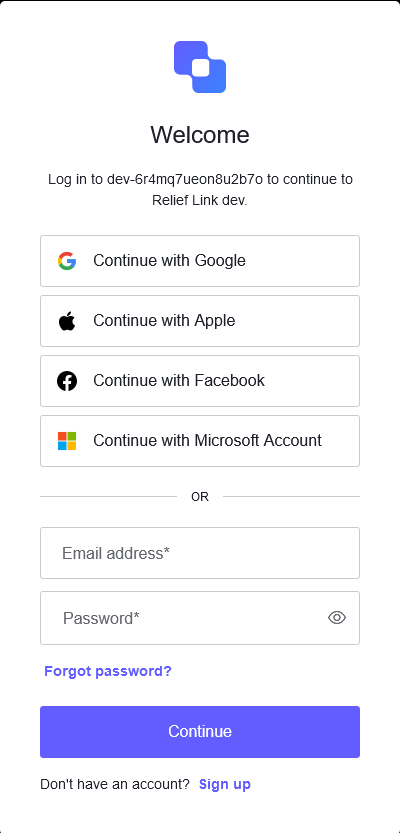
\includegraphics[width=\linewidth]{./figures/login.png}}
    \caption{Step 1: Login Page.}
    \label{fig:login}
\end{figure}

\begin{figure}[htbp]
    \centerline{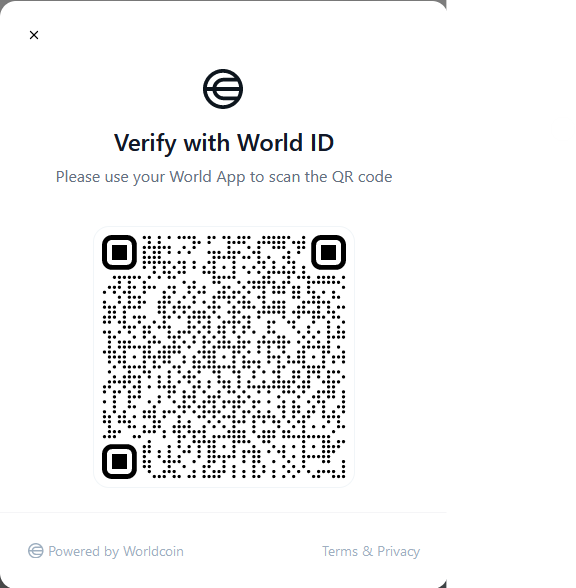
\includegraphics[width=\linewidth]{./figures/verify.png}}
    \caption{Step 2: Prove You Are Human by verifying with world ID.}
    \label{fig:verify}
\end{figure}

\begin{figure}[htbp]
    \centerline{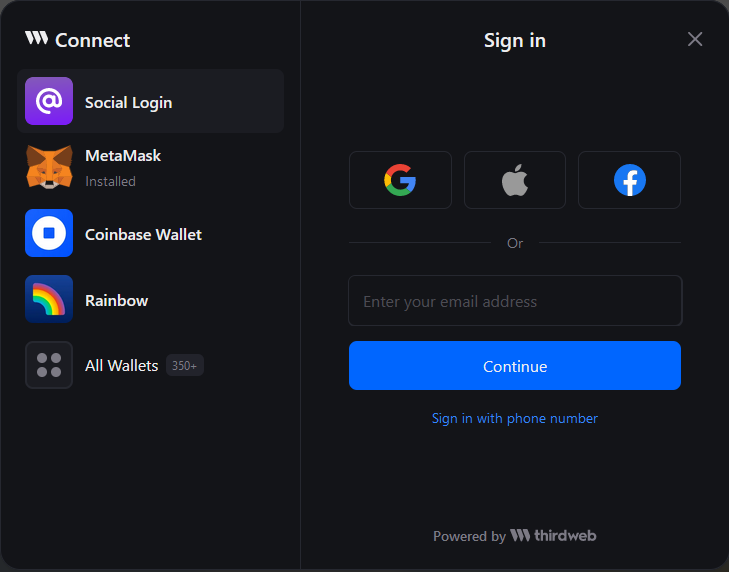
\includegraphics[width=\linewidth]{./figures/connect.png}}
    \caption{Step 3: Connect to your wallet.}
    \label{fig:connect}
\end{figure}

\begin{figure}[htbp]
    \centerline{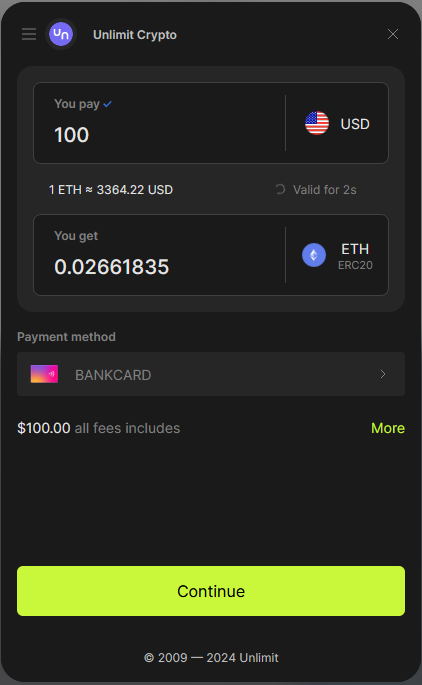
\includegraphics[width=\linewidth]{./figures/buy.png}}
    \caption{Step 3: Buy the cryptocurrency.}
    \label{fig:buy}
\end{figure}

\begin{figure}[htbp]
    \centerline{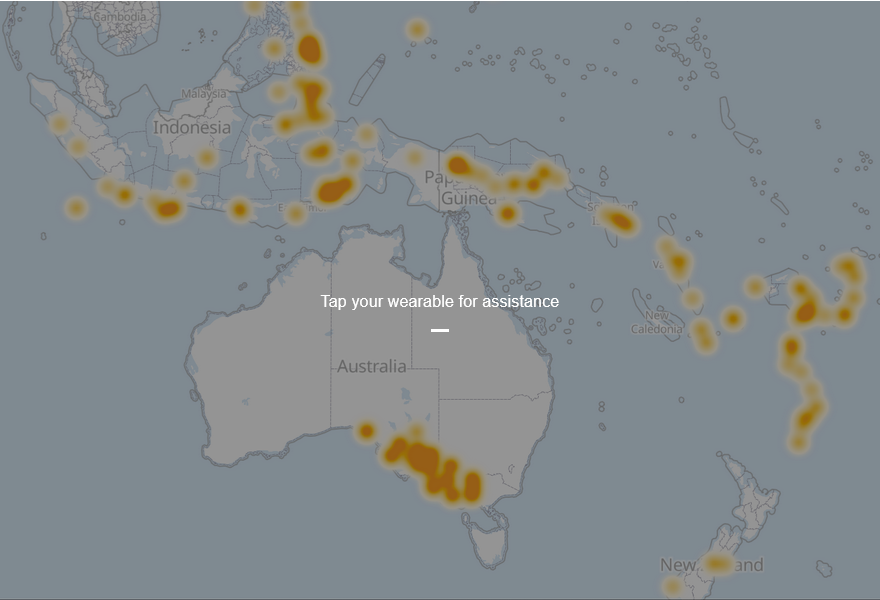
\includegraphics[width=\linewidth]{./figures/map.png}}
    \caption{Step 4: Set your residential address.}
    \label{fig:map}
\end{figure}

\end{document}
